\documentclass[12pt]{article}
\usepackage{times}
\usepackage[english]{babel}
\usepackage[utf8x]{inputenc}
\usepackage[colorinlistoftodos]{todonotes}
\usepackage[margin=1in]{geometry}
\usepackage{graphicx}
\usepackage{epstopdf}
\usepackage{cite}
\usepackage{listings}
\usepackage{dtklogos}
\usepackage{wrapfig}
\usepackage{subfigure}
\usepackage{amsmath}
\usepackage{amsthm}
\usepackage{amssymb}
\usepackage{amscd}
\usepackage{caption}
\usepackage{etoolbox}
\usepackage{fancyhdr}
\usepackage{stackengine}
\usepackage[export]{adjustbox}
\patchcmd{\thebibliography}{\section*{\refname}}{}{}{}
\usepackage[document]{ragged2e}    %This causes text to left align
\usepackage[colorlinks=true, linkcolor=black,citecolor=black,urlcolor=blue]{hyperref}
\bibliographystyle{IEEEtran}
\DeclareGraphicsRule{.tif}{png}{.png}{`convert #1 `dirname #1`/`basename #1 .tif`.png}

\title{MCHE 474: Lab 4}

\begin{document}
\lefthyphenmin3
\righthyphenmin4
% \pretolerance=2000
% \tolerance=500 
% \emergencystretch=10pt
%\raggedright     %Stops LaTeX from automatically hyphenating the right margin to fit better
%Combine this with \usepackage[document]{ragged2e} to get a text align left similar to natural MS Word


%-------------------------------------------------------------
%Start of Paper
%-------------------------------------------------------------

%%%%%%%%%%%%%%%%%%%%%%%%%%%%%%%%%%%%%%%%%%%%%%%%%%%%%%
%%%%%%%%%%%%%%%%%%%%%%% TITLE PAGE %%%%%%%%%%%%%%%%%%%%%%%%
%%%%%%%%%%%%%%%%%%%%%%%%%%%%%%%%%%%%%%%%%%%%%%%%%%%%%%

\begin{titlepage}

\newcommand{\HRule}{\rule{\linewidth}{0.5mm}} % Defines a new command for the horizontal lines, change thickness here

\center % Center everything on the page
 
%----------------------------------------------------------------------------------------
%	Heading Section
%----------------------------------------------------------------------------------------

\textsc{\LARGE University of Louisiana at Lafayette}\\[1.5cm] % Name of your university/college
\textsc{\Large Control Systems}\\[0.5cm] % Major heading such as course name
\textsc{\large MCHE 474}\\[0.5cm] % Minor heading such as course title

%----------------------------------------------------------------------------------------
%	Title Section
%----------------------------------------------------------------------------------------

\HRule \\[0.4cm]
{ \huge \bfseries Lab 4}\\[0.4cm] % Title of your document
\HRule \\[1.5cm]
 
%----------------------------------------------------------------------------------------
%	Author Section
%----------------------------------------------------------------------------------------

\begin{minipage}{0.4\textwidth}
\begin{flushleft} \large
\emph{Author:}\\
\textsc{Matthew J. Begneaud} \\% Your name
\end{flushleft}
\end{minipage}
~
\begin{minipage}{0.4\textwidth}
\begin{flushright} \large
\emph{Professor:} \\
\textsc{Dr. Mostafa A. Elsayed} % Supervisor's Name
\end{flushright}
\end{minipage}\\[1.5cm]

% If you don't want a supervisor, uncomment the two lines below and remove the section above
%\Large \emph{Author:}\\
%John \textsc{Smith}\\[3cm] % Your name

%----------------------------------------------------------------------------------------
%	Date Section
%----------------------------------------------------------------------------------------

{\textsc{\large \today}}\\[2cm] % Date, change the \today to a set date if you want to be precise

%----------------------------------------------------------------------------------------
%	Logo Section
%----------------------------------------------------------------------------------------


\includegraphics[width=5in]{UL_logo.jpg}\\[1cm] % Include a department/university logo - this will require the graphicx package
 
%----------------------------------------------------------------------------------------

\vfill % Fill the rest of the page with whitespace

\end{titlepage}

%%%%%%%%%%%%%%%%%%%%%%%%%%%%%%%%%%%%%%%%%%%%%%%%%%%%%%
%%%%%%%%%%%%%%%%%%%%%%% TABLE OF CONTENTS %%%%%%%%%%%%%%%%%%%
%%%%%%%%%%%%%%%%%%%%%%%%%%%%%%%%%%%%%%%%%%%%%%%%%%%%%%

\tableofcontents

\listoffigures

\section*{\fontsize{12}{12}\selectfont \large List of Symbols}
\addcontentsline{toc}{section}{List of Symbols} % Add for each section
$G$ = Plant function \\
$s$ = Laplace Domain variable \\
$PID$ = Proportional-Integral-Derivative Controller \\
$KP$ = Proportional Gain \\
$KI$ = Integral Gain \\
$KD$ = Derivative Gain \\

\newpage

%%%%%%%%%%%%%%%%%%%%%%%%%%%%%%%%%%%%%%%%%%%%%%%%%%%%%%
%%%%%%%%%%%%%%%%%%%%%%% REPORT %%%%%%%%%%%%%%%%%%%%%%%%%%
%%%%%%%%%%%%%%%%%%%%%%%%%%%%%%%%%%%%%%%%%%%%%%%%%%%%%%


\section*{\fontsize{12}{12}\selectfont \large Introduction}
\addcontentsline{toc}{section}{Introduction} % Add for each section
This lab was conducted using MATLAB in order to analyze control systems. The plant function for the second order system analyzed in this lab is given, and is shown in Equation 1. The main aspect of the system analyzed in this lab is the effect of a proportional, integral, and derivative control (PID controller).

\begin{equation}
G = \frac{50}{s^{2}+30s+75}
\end{equation}



\section*{\fontsize{12}{12}\selectfont \large Theory}
\addcontentsline{toc}{section}{Theory} % Add for each section
A PID is a feedback controller which accounts for not just one state of error, but three, in order to modify the input to the system to achieve the desired state. The equation for a PID controller is shown in Equation 2, and is rewritten in Equation 3.
\bigskip

\begin{equation}
PID= KP + KI/S + KD S 
\end{equation}

\begin{equation}
PID= (KD S^2 + KP S + KI)/S
\end{equation}
\bigskip

The effect of the proportional, integral, and derivative components of the controller are weighted by their gains $KP$, $KI$, and $KD$ respectively. Adjusting these gains allows for the PID controller to be tailored to fit the system and the desired performance. Adjusting the proportional gain changes how intensely the controller reacts to error. Adjusting the integral gain changes how quickly accumulated error is accounted for by increasing the controller output. Adjusting the derivative gain changes how quickly the controller reacts to a change in the rate of error change, which is useful for situations where the error changes signs frequently (like an autonomous vehicle which needs to stick to a straight course).
\bigskip

In general, an increase in $KP$ results in a decrease in rise time, increase in overshoot, and a decrease in steady-state error. An increase in $KI$ results in a decrease in rise time, increase in overshoot, and an elimination of steady-state error (because the integral component adjusts the controller output to overcome and error that is failing to change) at the cost of an increase in settling time. An increase in $KD$ results in a decrease in overshoot and a decrease in settling time.



\section*{\fontsize{12}{12}\selectfont \large Procedure \& Analysis}
\addcontentsline{toc}{section}{Procedure \& Analysis} % Add for each section
The system was simulated in MATLAB and a PID controller was implemented. First values of $KP=1$, $KI=KD=0$ were used for the controller. The $KP$ was then changed to values of 2 and 10. The system responses for all three combinations are shown in Figure 1. The system characteristics of each combination are shown in Figure 2 through Figure 4. Notice that the increase in $KP$ causes an increase in amplitude and overshoot.

\newpage

\begin{figure}[h!] %  figure placement: here, top, bottom, or page
   \centering
   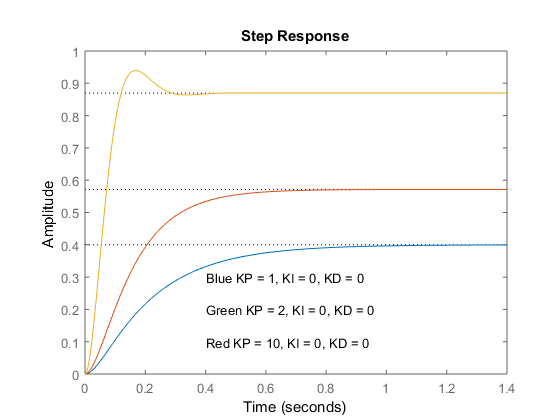
\includegraphics[width=\linewidth]{part_1_response.png} 
   \caption{Varying $KP$ System Response}
   \label{fig:example}
\end{figure}

\bigskip

\begin{figure}[h!] %  figure placement: here, top, bottom, or page
   \centering
   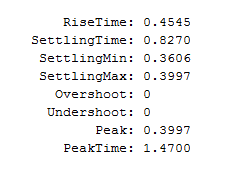
\includegraphics[width=3in]{1_100.png} 
   \caption{$KP = 1$, $KI = KD = 0$}
   \label{fig:example}
\end{figure}

\newpage

\begin{figure}[h!] %  figure placement: here, top, bottom, or page
   \centering
   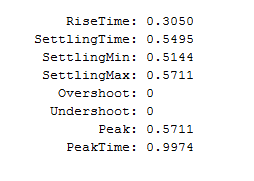
\includegraphics[width=3in]{1_200.png} 
   \caption{$KP = 2$, $KI = KD = 0$}
   \label{fig:example}
\end{figure}

\bigskip

\begin{figure}[h!] %  figure placement: here, top, bottom, or page
   \centering
   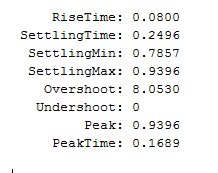
\includegraphics[width=3in]{1_1000.png} 
   \caption{$KP = 10$, $KI = KD = 0$}
   \label{fig:example}
\end{figure}

\bigskip
\bigskip

Second, values of $KP=1$, $KI=KD=0$ were used for the controller. The $KI$ was then changed to values of 10 and 30. The system responses for all three combinations are shown in Figure 5. The system characteristics of each combination are shown in Figure 6 through Figure 8. Notice that the increase in $KI$ causes an increase in overshoot and settling time, while decreasing the rise time.

\newpage

\begin{figure}[h!] %  figure placement: here, top, bottom, or page
   \centering
   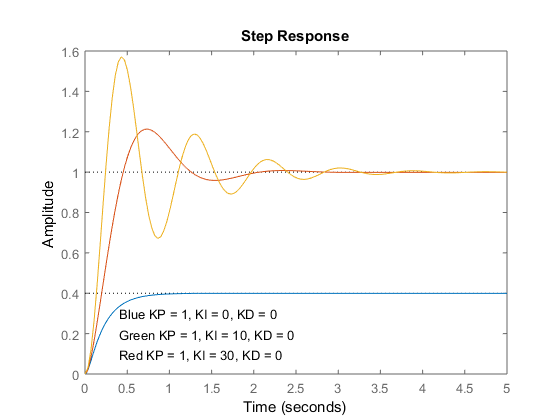
\includegraphics[width=\linewidth]{part_2_response.png} 
   \caption{Varying $KI$ System Response}
   \label{fig:example}
\end{figure}

\bigskip

\begin{figure}[h!] %  figure placement: here, top, bottom, or page
   \centering
   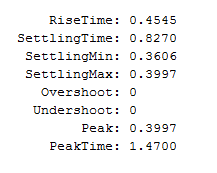
\includegraphics[width=3in]{2_100.png} 
   \caption{$KP = 1$, $KI = 0$, $KD = 0$}
   \label{fig:example}
\end{figure}

\newpage

\begin{figure}[h!] %  figure placement: here, top, bottom, or page
   \centering
   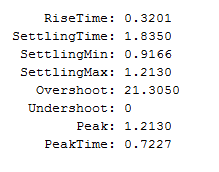
\includegraphics[width=3in]{2_1100.png} 
   \caption{$KP = 1$, $KI = 10$, $KD = 0$}
   \label{fig:example}
\end{figure}

\bigskip

\begin{figure}[h!] %  figure placement: here, top, bottom, or page
   \centering
   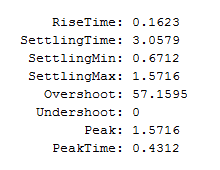
\includegraphics[width=3in]{2_1300.png} 
   \caption{$KP = 1$, $KI = 30$, $KD = 0$}
   \label{fig:example}
\end{figure}

\bigskip
\bigskip

Third, values of $KP=1$, $KI=30$, $KD=0$ were used for the controller. The $KD$ was then changed to values of 2 and 10. The system responses for all three combinations are shown in Figure 9. The system characteristics of each combination are shown in Figure 10 through Figure 12. Notice that the increase in $KD$ causes an decrease in overshoot and settling time.

\newpage

\begin{figure}[h!] %  figure placement: here, top, bottom, or page
   \centering
   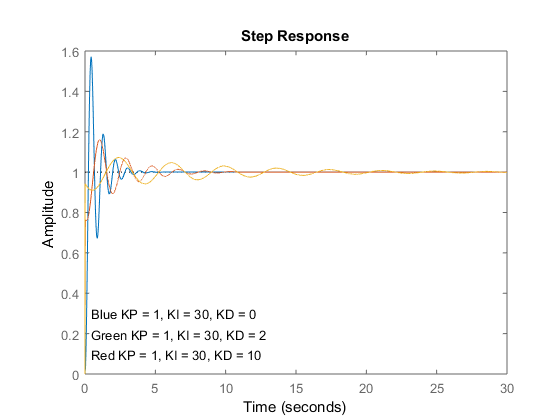
\includegraphics[width=\linewidth]{part_3_response.png} 
   \caption{Varying $KD$ System Response}
   \label{fig:example}
\end{figure}

\bigskip

\begin{figure}[h!] %  figure placement: here, top, bottom, or page
   \centering
   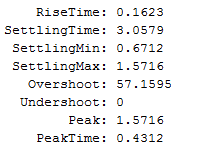
\includegraphics[width=3in]{3_1300.png} 
   \caption{$KP = 1$, $KI = 30$, $KD = 0$}
   \label{fig:example}
\end{figure}

\newpage

\begin{figure}[h!] %  figure placement: here, top, bottom, or page
   \centering
   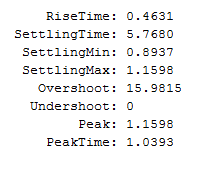
\includegraphics[width=3in]{3_1302.png} 
   \caption{$KP = 1$, $KI = 30$, $KD = 2$}
   \label{fig:example}
\end{figure}

\bigskip

\begin{figure}[h!] %  figure placement: here, top, bottom, or page
   \centering
   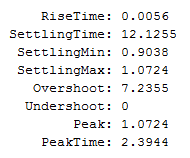
\includegraphics[width=3in]{3_13010.png} 
   \caption{$KP = 1$, $KI = 30$, $KD = 10$}
   \label{fig:example}
\end{figure}

\bigskip

Fourth, values of $KP=1$, $KI=0$, $KD=0$ were used for the controller. The $KI$ was then changed to a value of 30, and then the $KD$ was changed to a value of 10. This combination of gains allows us to compare the effects of adding each component additionally to the controller. The system responses for all three combinations are shown in Figure 13. The system characteristics of each combination are shown in Figure 14 through Figure 16. Notice that the addition of integral control raises the overshoot and settling time, which is then decreased by adding a derivative component to the controller.

\newpage

\begin{figure}[h!] %  figure placement: here, top, bottom, or page
   \centering
   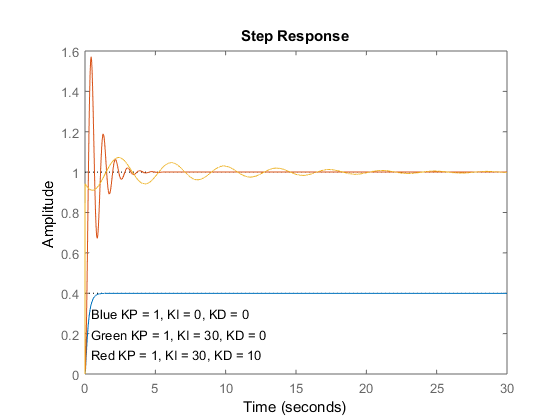
\includegraphics[width=\linewidth]{part_4_response.png} 
   \caption{Sequential Addition of Components to Controller System Response}
   \label{fig:example}
\end{figure}

\bigskip

\begin{figure}[h!] %  figure placement: here, top, bottom, or page
   \centering
   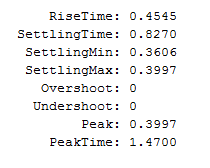
\includegraphics[width=3in]{4_100.png} 
   \caption{$KP = 1$, $KI = 30$, $KD = 0$}
   \label{fig:example}
\end{figure}

\newpage

\begin{figure}[h!] %  figure placement: here, top, bottom, or page
   \centering
   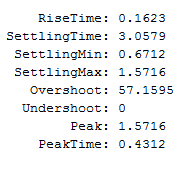
\includegraphics[width=3in]{4_1300.png} 
   \caption{$KP = 1$, $KI = 30$, $KD = 2$}
   \label{fig:example}
\end{figure}

\bigskip

\begin{figure}[h!] %  figure placement: here, top, bottom, or page
   \centering
   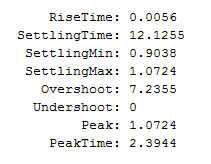
\includegraphics[width=3in]{4_13010.png} 
   \caption{$KP = 1$, $KI = 30$, $KD = 10$}
   \label{fig:example}
\end{figure}



\section*{\fontsize{12}{12}\selectfont \large Conclusion}
\addcontentsline{toc}{section}{Conclusion} % Add for each section
The exercises conducted in this lab reinforce the theory learned in the classroom. It is shown
that systems can be controlled using a PID controller, which is a tunable feedback controller which accounts for present, past, and future error states of the system. PID controllers are used widely in industrial applications, and this experience of adjusting a PID controller's gains and observing the effects on the controller is extremely useful to engineering students.




%\section*{\fontsize{12}{12}\selectfont \large References}

\begin{thebibliography}{2}

% Example
%\bibitem{Wagner}
%Ng, K., Wagner, S.W., Camelio, J., Emblom, W.J. (2010). ?Experimental Analysis of Micro Tube
%Hydroforming Process.? Transactions of NAMRC of SME, 38, 577-584.

\end{thebibliography}



%\section*{\fontsize{12}{12}\selectfont APPENDIX}

%\begin{table}[h!]
%  \caption{}
%  \includegraphics[width=\linewidth]{table1.png}
%\end{table}




\end{document}







----------------------------Templates-------------------------------

-------------------------Figure-----------------------

\begin{figure}[h!]  
  \centering
    \includegraphics[width=\linewidth]{**file**}
    \caption{Docking Station}
\end{figure}

---------------------------Table-----------------------
\begin{table}[ht]
\caption{Nonlinear Model Results} % title of Table
\centering % used for centering table
\begin{tabular}{c c c c} % centered columns (4 columns)
\hline\hline %inserts double horizontal lines
Case & Method\#1 & Method\#2 & Method\#3 \\ [0.5ex] % inserts table
%heading
\hline % inserts single horizontal line
1 & 50 & 837 & 970 \\ % inserting body of the table
2 & 47 & 877 & 230 \\
3 & 31 & 25 & 415 \\
4 & 35 & 144 & 2356 \\
5 & 45 & 300 & 556 \\ [1ex] % [1ex] adds vertical space
\hline %inserts single line
\end{tabular}
\label{table:nonlin} % is used to refer this table in the text
\end{table}



probably best to insert as an image from excel

\bigskip\\
\begin{table}[h!]
  \caption{}
  \includegraphics[width=\linewidth]{**file**}
\end{table}
\bigskip\\





-----------------------------Equations------------------------
-----------------------------Regular
\begin{equation}
a = b + c
\end{equation}

--------------------------------- Multiline
\begin{multline}
a = b + c + d + e + f
+ g + h + i + j \\
+ k + l + m + n + o
\end{multline}

-------------------------------Citations-------------------------
\bibitem{Author last name}
  Last, First., year of publication,
  article name, book(etc) name, from \\
  link goes here

----------------------------------other-----------------------------

equations:
http://moser-isi.ethz.ch/docs/typeset_equations.pdf

citations:
http://library.missouri.edu/engineering/about/guides/asme
https://www.asme.org/shop/proceedings/conference-publications/references